\section{SCGRA Compilation} \label{sec:scgracompile}
\subsection{Overview Of SCGRA Compilation}
\figref{fig:scgra-compile} illustrates the detailed SCGRA compilation of QuickDough. As shown in the diagram, it aims to compile a compute kernel of an application to a customized SCGRA and generate the corresponding implementation bitstream. 
 
\begin{figure}[htb]
\center{\includegraphics[width=0.65\linewidth]{scgra-compile}}
\caption{SCGRA Compilation}
\label{fig:scgra-compile}
\end{figure}

The compilation starts from transforming the compute kernel probably written in high level language to a DFG as well as hyper block which is a number of consecutive DFG. Given the DFG and block, a customized SCGRA configuration based on the template presented in previous section is determined. Then the DFG and block can be scheduled to the specified SCGRA using an operation scheduler. As the simulation performance of the DFG and block can be acquired from the scheduling, with the pre-built SCGRA implementation frequency and the communication efficiency of the compute system, we can obtain even accurate performance of the compute kernel and can further check whether the performance goal is met. If the design goal is not met, we can go back to the block and DFG generation stage altering the design options such as loop unrolling factor. Repeat these steps until the design goal is achieved.

Once the design goal is met, the configuration words can be extracted from the scheduler and be integrated into the pre-built SCGRA bitstream using the data2mem tool. Since the bitstream in the SCGRA library is bundled with specific FPGA device, HDL model will be used for porting to a new device and complete hardware implementation flow is required accordingly.

\subsection{Block and DFG Generation}
The communication between the processor and the accelerator is costly. When the data size of a DFG is small, data transmission for each DFG execution may compromise all the benefits of the accelerator. To solve this problem, we have the accelerator to repeat the DFG execution multiple times and combine them as a block. Data transmission is performed with the granularity of a block instead of a DFG which helps to amortize the initial communication overhead especially for the DMA transmission. \figref{fig:blocking-and-dfg-gen} shows the relation among the compute kernel, block and DFG using a simple example. 

\begin{figure}[htb]
\center{\includegraphics[width=1\linewidth]{dfg-gen}}
\caption{Relation of Compute Kernel, Block and DFG}
\label{fig:blocking-and-dfg-gen}
\end{figure}

Since the SCGRA employs lock-step execution and the input/output data for each block execution must also be fully buffered, the block size is mainly limited by the data buffer size. Given the block size, we need further to decide the loop unrolling factor such that the unrolled part can be transformed to DFG which can be executed on the SCGRA. Usually, the unrolling factor is limited by the instruction memory and data memory. 

In addition, we have straightforward address buffers which store all the on chip buffer accessing addresses of the whole block execution. Although it is already set to be twice larger than the data buffer, it still overflows easily and becomes another major limitation of both the block size and the unrolling factor. Finally, the compute kernel depends on the repeating of the block execution and the block execution depends on the repeating of the DFG execution. As a result, the loop count must be fully divided by the block size and the block size must also be fully divided by the unrolling factor. This can be another unrolling and blocking limitation as well. 

\subsection{SCGRA Customization}
There are a lot of SCGRA design parameters such as operation type, SCGRA size, SCGRA topology and the number of data buffers to be customized. However, we are not going to solve all the customization problems in this work. Instead, we mainly provide implementations of a few different customized SCGRAs and investigate how the \emph{softness} of SCGRA impacts on the overall performance and overhead. In this work, we implemented SCGRAs with different SCGRA size and operation type, while the rest design parameters are fixed. 
   
\subsection{Operation Scheduler}
The operation scheduler adopts a classical list scheduling algorithm \cite{schutten1996list} to tackle the DFG scheduling. While scheduling operations to PEs closer with each other could reduce the communication cost but may lose the load balance, a scheduling metric compromising both the communication and load balance as presented in \cite{colinheart} is delicately adjusted to adapt to the proposed SCGRA overlay.    

\begin{algorithm}
\caption{The SCGRA scheduling algorithm.}
\label{alg:scheduling}
\begin{algorithmic}
\PROCEDURE{ListScheduling}
\STATE Initialize the operation ready list $L$
\WHILE {$L$ is not empty}
\STATE select a PE $p$
\STATE select an operation $l$
\STATE OPScheduling($p$, $l$)
\STATE Update $L$
\ENDWHILE
\ENDPROCEDURE
\STATE
\PROCEDURE {OPScheduling($p$,$l$)}
\FORALL {predecessor operations $s$ of $l$}
\STATE Find nearest PE $q$ that has a copy of operation $s$
\STATE Find shortest routing path from PE $q$ to PE $p$
\STATE Move operation $s$ from PE $q$ to PE $p$ along the path
\ENDFOR
\STATE Do operation $l$ on PE $p$
\ENDPROCEDURE

\end{algorithmic}
\end{algorithm}

\algref{alg:scheduling} briefly illustrates the scheduling algorithm implemented in QuickDough. Initially, an operation ready list is created to store operations that can be scheduled. The next step is to select a PE from the SCGRA and an operation from the operation ready list using the compromised communication and load balance metric. When both the PE and the operation to be scheduled are determined, the OPScheduling procedure starts. It will figure out an optimized routing path, move the source operands to the selected PE along the path, and have the selected operation executed accordingly. After this step, the operation ready list is updated as the latest scheduling may produce more ready operations. Repeat the OPScheduling procedure as well as the operation ready list updating. The DFG scheduling will be completed when the operation ready list is empty. Finally, the control words of each PE and the IO buffer accessing sequence will be dumped from the scheduler. They will be used for bitstream generation in the following compilation step. 

\subsection{Bitstream Integration}
The final step of the compilation is to incorporate the instruction for each PE as well as the IO buffer addresses obtained from the scheduling result with the pre-compiled SCGRA bitstream. By design, our SCGRA does not have mechanism to load instruction streams from external memory. Instead, we take advantage of the reconfigurability of SRAM based FPGAs and store the cycle-by-cycle configuration words using on-chip ROMs. The content of the ROMs are embedded in the bitstream and data2mem tool from Xilinx \cite{data2mem} can be used to update the ROM content of the pre-built bitstream directly. To complete the bitstream integration, BMM file that describes the organization and placed location of the ROMs in SCGRA overlay is also required and it can be extracted from the XDL file \cite{beckhoff2011xilinx} of the pre-built SCGRA overlay automatically. While original SCGRA design needs around an hour to implement, the bitstream integration only costs a few seconds.
